\documentclass[laporan.tex]{subfiles}

\begin{document}

\chapter{Tinjauan Pustaka}

\section{Penelitian Terkait}

\subsection{Improving quality inspection of food products by computer vision – a review}

Kualitas produk pangan diukur dari penampilan, bau, tekstur, rasa dan berbagai aspek subjektif lainnya yang dinilai oleh manusia. Namun inspeksi dengan tenaga manusia mempunyai banyak kelemahan antara lain ongkos yang tinggi serta  hasil yang tidak konsisten.

Makalah ini\cite{brosnan} membahas berbagai penelitian di bidang computer vision yang diterapkan untuk menggantikan inspeksi manual pada berbagai produk pangan dan pertanian.

Beberapa penelitian memfokuskan pada deteksi cacat bentuk atau tekstur secara visual. Ekspansi Fourier dapat mendeteksi bentuk kultivar apel dengan kesuksesan 90\%.

\subsection{Navel Orange Blemish Identification for Quality Grading System}

Menurut penelitian ini, klasifikasi pixel untuk mengenali memar pada kulit jeruk mempunyai akurasi rendah karena perbedaan intensitas warna antara bagian tengah jeruk dengan bagian tepi jeruk pada citra jeruk. Untuk mengatasi masalah tersebut pengetahuan a priori mengenai variasi intensitas pada benda bulat diterapkan agar pixel bagian yang cacat dapat dikenali dengan tepat.\cite{liu}

Sistem deteksi cacat berusaha meniru persepsi manusia yang membandingkan warna secara relatif dengan warna sekeliling.

Langkah pertama deteksi adalah dengan menggolongkan jeruk berdasarkan kematangan. Algoritma yang digunakan berbeda untuk jeruk matang dan mentah karena adanya variasi warna pada jeruk mentah. Klasifikasi ini dilakukan dengan selisih nilai \emph{threshold} Otsu pada komponen warna merah dan hijau. Jeruk matang mempunyai nilai selisih yang lebih tinggi.

Klasifikasi awal dilakukan pada warna-warna kulit jeruk berdasarkan nilai komponen R, G dan B pada tiap pixel. Nilai yang kurang dari ambang batas berdasarkan algoritma Otsu dianggap tidak ada pada pixel. Berdasarkan kombinasi warna primer, tiap pixel digolongkan menjadi satu dari delapan jenis warna.

\begin{tabular}{|c|c|c|c|c|}
\hline
No. & Kelas Warna & R & G & B \\
\hline
1. & Latar belakang & 0 & 0 & 0 \\
2. & Biru & 0 & 0 & 1 \\
3. & Hijau & 0 & 1 & 0 \\
4. & Cyan & 0 & 1 & 1 \\
5. & Merah & 1 & 0 & 0 \\
6. & Magenta & 1 & 0 & 1 \\
7. & Kuning & 1 & 1 & 0 \\
8. & Putih & 1 & 1 & 1 \\
\hline
\end{tabular}

Kelas-kelas tersebut diberi bobot sedemikian rupa sehingga terurut dari intensitas terendah sampai intensitas tertinggi. Hasil eksperimen menunjukkan bahwa kelas warna merah dan magenta tidak ditemukan pada jeruk matang maupun mentah.

Selanjutnya untuk tiap kelas dihitung intensitas rata-rata pada masing-masing komponen warna primer. Jarak antarkelas dihitung dengan \emph{squared mean difference} dari rata-rata intensitas untuk masing-masing komponen, kemudian dirata-rata dengan \emph{quadratic mean}. Dari jarak antarkelas dapat ditemukan adanya beberapa kelas yang bertetangga, yaitu dua kelas yang terdekat satu sama lain. Kelas yang bertetangga digabungkan menjadi kelas baru, sedangkan kelas yang tidak ada pada data dihapus. Dilakukan perhitungan rata-rata intensitas pada kelas baru.

Klasifikasi selanjutnya dilakukan dengan pencarian jarak minimum dari tiap pixel dengan rata-rata intensitas masing-masing kelas baru. Pixel yang masuk pada kelas dengan intensitas tertinggi (\emph{top layer}) dianggap sebagai bagian kulit jeruk yang normal, sedangkan bagian cacat ditentukan dari lubang pada daerah dengan intensitas tertinggi tersebut.

Metode di atas dapat menentukan daerah cacat sebanyak 70\%-80\% pada bagian tengah dari seluruh permukaan jeruk yang tampak pada citra. Deteksi tidak dapat dilakukan pada bagian tepi karena adanya perbedaan intensitas cahaya yang diterima oleh objek.

\section{Computer Vision}

Citra digital adalah fungsi intensitas warna dua dimensi $f(x,y)$, dengan $x$ dan $y$ mewakili koordinat lokasi suatu titik dan nilai dari fungsi yang merupakan tingkat intensitas warna atau tingkat keabu-abuan dari titik tersebut (Schalkoff, 1989). Citra digital merupakan representasi dari suatu objek nyata yang dapat dikenali oleh komputer.

Pengolahan citra digital atau digital image processing pengolahan sinyal untuk input citra digital dua dimensi. Tujuan pengolahan citra digital adalah untuk meningkatkan kualitas gambar sehingga lebih mudah dilihat oleh manusia atau lebih mudah diolah oleh komputer.

Computer vision adalah bidang studi yang mempelajari metode-metode pengumpulan, pemrosesan, analisis dan penafsiran citra dari dunia nyata dengan tujuan untuk menghasilkan informasi numerik atau simbolis.

Berikut ini adalah pengertian computer vision menurut beberapa pakar

\begin{enumerate}
\item Ballard dan Brown, computer vision adalah otomatis dan integrasi sebuah range yang luas yang terdiri dari proses-proses dan representasi-representasi terhadap persepsi visual.
\item Adrian Low, computer vision berhubungan dengan perolehan gambar, pemrosesan, klasifikasi, pengenalan, dan menjadi penggabungan, pengurutan, pembuatan keputusan menuju pengenalan.
\item Shapiro dan Stockman, computer vision adalah suatu bidang yang bertujuan untuk membuat suatu keputusan yang berguna mengenai objek fisik nyata dan keadaan berdasarkan atas sebuah citra. Computer vision merupakan kombinasi antara pengolahan citra dan pengenalan pola. Hasil keluaran dari proses computer vision adalah pengertian tentang citra.
\end{enumerate}

Boyle dan Thomas mengatakan bahwa computer vision lebih daripada pengenalan, computer vision melakukan operasi “low level processing” sebagai algoritma image processing yang murni. Mereka juga yang menggolongkan image processing ke dalam computer vision.

\section{Metode Otsu}

Metode segmentasi Otsu digunakan untuk memisahkan pixel latar belakang dengan pixel objek. Algoritma Otsu membagi data histogram menjadi dua kelas dengan mencari nilai ambang yang memaksimumkan selisih rata-rata data antarkelas, dengan demikian memperkecil selisih rata-rata data dalam satu kelas. Perhitungan tersebut diformulasikan sebagai berikut

\begin{equation}
	\sigma_{\omega}^2 (t) = \omega_1 (t) \sigma_{\omega}^2 (t) + \omega_2 (t) \sigma_{\omega}^2 (t)
\end{equation}

Algoritma secara umum
\begin{enumerate}
\item Hitung probabilitas tiap nilai \emph{grayscale}
\begin{equation}
	p_i = \frac{n_i}{t_n}
\end{equation}
\item Mulai dengan intensitas \emph{grayscale} terendah $t=minGL$, bagi data menjadi dua kelas dengan nilai $minGL \ldots t$ dan $t \ldots maxGL$. Hitung probabilitas tiap kelas.
\begin{align}
	\omega_1 = & \sum_{i=minGL}^t p_i \\
	\omega_2 = & \sum_{i=t+1}^{maxGL} p_i
\end{align}
\item Hitung rata-rata masing-masing kelas.
\begin{align}
	\mu_1 = & \frac{\sum_{i=minGL}^t p_i}{\omega_1} \\
	\mu_2 = & \frac{\sum_{i=t+1}^{maxGL} p_i}{\omega_2}
\end{align}
\item Hitung variansi untuk masing-masing kelas.
\begin{align}
	\sigma_1^2 = & \frac{\sum_{i=minGL}^t (i - \mu_1)^2 p_i}{\omega_1} \\
	\sigma_2^2 = & \frac{\sum_{i=t+1}^{maxGL} (i - \mu_2)^2 p_i}{\omega_2}
\end{align}
\item Hitung jumlah variansi kedua kelas.
\begin{equation}
	\sigma_{\omega}^2 = \omega_1 \sigma_1^2 + \omega_2 \sigma_2^2
\end{equation}
\item Ulangi untuk setiap nilai antara $minGL \ldots maxGL$.
\item Nilai \emph{threshold} optimum adalah yang menghasilkan nilai $\sigma_{\omega}^2$ minimum.
\end{enumerate}

\section{Perhitungan Jarak Euclidean}

Ukuran perbedaan antara titik-titik data dengan $n$-atribut dapat dideskripsikan sebagai jarak antardata pada ruang Euclidean dimensi-$n$. Salah satu perhitungan yang digunakan untuk mengukur jarak antardata adalah rumus Euclid.

\begin{equation}
	d=\sqrt{\sum_{i=1}^n (a_i - b_i)^2}
\end{equation}

$a_i$ dan $b_i$ adalah atribut ke-$i$ dari $a$ dan $b$.

Perhitungan jarak Euclidean digunakan untuk mendapatkan kelas-kelas warna yang bertetangga mengklasifikasikan pixel pada tahap klasifikasi ke dua.

%\section{Operasi Morfologi \emph{Convex Hull}}

%\emph{Convex hull} $H$ dari himpunan sembarang $S$ adalah himpunan \emph{convex} terkecil yang mengandung semua elemen $S$. Himpunan $H$ merupakan himpunan \emph{convex} jika semua garis lurus yang menghubungkan elemen $A$ dan $B$ pada himpunan $H$ terletak seluruhnya pada $H$. Selisih himpunan $H - S$ disebut sebagai \emph{convex deficiency} dari $S$.

\section{Deteksi dan Pengukuran Prosentase Cacat Kulit Jeruk}

%Pada metode klasifikasi yang diujicobakan ini, \emph{pixel} yang masuk pada kelas dengan intensitas rata-rata tertinggi dianggap sebagai daerah normal kulit jeruk. Daerah cacat ditemukan dari \emph{convex deficiency} kumpulan \emph{pixel} dengan intensitas tertinggi. Prosentase cacat merupakan perbandingan antara \emph{convex hull} dari area dengan \emph{pixel} normal dengan \emph{convex deficiency}.

Cacat kulit jeruk terdeteksi sebagai lubang-lubang pada \emph{mask} yang dibentuk dari \emph{pixel} yang diklasifikasikan dalam dengan intensitas rata-rata tertinggi.

\begin{align}
	p_{cacat} = & \frac{L_{cacat}}{L_{normal} + L_{cacat}} \\
	L_{normal} \approx & Luas(H) \\
	L_{cacat} \approx & Luas(H - H)'
\end{align}

%$H'$ adalah \emph{convex hull} semua \emph{pixel} $H$ yang masuk dalam kelas dengan intensitas tertinggi.
$H$ adalah kumpulan \emph{pixel} dengan kelas yang paling tinggi intensitasnya, $H'$ adalah hasil pengisian lubang. Cacat dideteksi dari selisih antara $H$ dan $H'$.

\section{Akurasi Deteksi}

Akurasi deteksi cacat akan diukur dari parameter presisi, \emph{recall} dan akurasi statistik jumlah \emph{pixel} daerah cacat dan daerah normal.

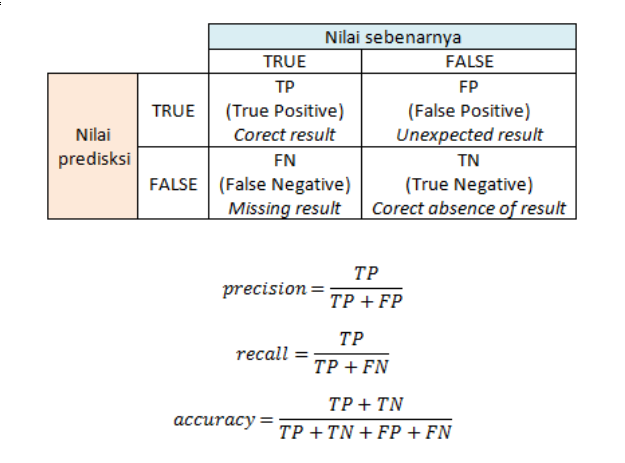
\includegraphics[width=8cm]{tex/conf.png}

Selain itu ditambahkan lagi ukuran kemampuan deteksi yang dirumuskan sebagai perbandingan antara luas daerah yang dapat diproses dari tiap citra jeruk dengan luas keseluruhan objek jeruk yang tampak.

\begin{equation}
	deteksi = \frac{Luas(H')}{\sum_{kelas>1}^n Luas(M_{kelas})}
\end{equation}

$H'$ merupakan hasil pengisian lubang yang menunjukkan bagian yang dapat diproses, $M_{kelas}$ merupakan mask hasil klasifikasi akhir jeruk.

\end{document}
